%%%%%%%%%%%%%%%%%%%%%%%%%%%%%%%%%%%%%%%%%%%%%%%%%%%%%%%%%%%%%%%%%%%%%
%%                                                                 %%
%% Please do not use \input{...} to include other tex files.       %%
%% Submit your LaTeX manuscript as one .tex document.              %%
%%                                                                 %%
%% All additional figures and files should be attached             %%
%% separately and not embedded in the \TeX\ document itself.       %%
%%                                                                 %%
%%%%%%%%%%%%%%%%%%%%%%%%%%%%%%%%%%%%%%%%%%%%%%%%%%%%%%%%%%%%%%%%%%%%%

%%\documentclass[referee,sn-basic]{sn-jnl}% referee option is meant for double line spacing

%%=======================================================%%
%% to print line numbers in the margin use lineno option %%
%%=======================================================%%

%%\documentclass[lineno,sn-basic]{sn-jnl}% Basic Springer Nature Reference Style/Chemistry Reference Style

%%======================================================%%
%% to compile with pdflatex/xelatex use pdflatex option %%
%%======================================================%%

%%\documentclass[pdflatex,sn-basic]{sn-jnl}% Basic Springer Nature Reference Style/Chemistry Reference Style
%%\documentclass[sn-basic]{sn-jnl}% Basic Springer Nature Reference Style/Chemistry Reference Style
%%\documentclass[sn-mathphys]{sn-jnl}% Math and Physical Sciences Reference Style
%%\documentclass[sn-aps]{sn-jnl}% American Physical Society (APS) Reference Style
%%\documentclass[sn-vancouver]{sn-jnl}% Vancouver Reference Style
%%\documentclass[sn-apa]{sn-jnl}% APA Reference Style
%%\documentclass[sn-chicago]{sn-jnl}% Chicago-based Humanities Reference Style
%%\documentclass[sn-standardnature]{sn-jnl}% Standard Nature Portfolio Reference Style
%%\documentclass[default]{sn-jnl}% Default
\documentclass[default,iicol]{sn-jnl}% Default with double column layout

%%%% Standard Packages
%%<additional latex packages if required can be included here>
%%%%

%%%%%=============================================================================%%%%
%%%%  Remarks: This template is provided to aid authors with the preparation
%%%%  of original research articles intended for submission to journals published 
%%%%  by Springer Nature. The guidance has been prepared in partnership with 
%%%%  production teams to conform to Springer Nature technical requirements. 
%%%%  Editorial and presentation requirements differ among journal portfolios and 
%%%%  research disciplines. You may find sections in this template are irrelevant 
%%%%  to your work and are empowered to omit any such section if allowed by the 
%%%%  journal you intend to submit to. The submission guidelines and policies 
%%%%  of the journal take precedence. A detailed User Manual is available in the 
%%%%  template package for technical guidance.
%%%%%=============================================================================%%%%

\jyear{2022}%
\usepackage{lmodern}%%
\usepackage{stfloats}

%% as per the requirement new theorem styles can be included as shown below
\theoremstyle{thmstyleone}%
\newtheorem{theorem}{Theorem}%  meant for continuous numbers
%%\newtheorem{theorem}{Theorem}[section]% meant for sectionwise numbers
%% optional argument [theorem] produces theorem numbering sequence instead of independent numbers for Proposition
\newtheorem{proposition}[theorem]{Proposition}% 
%%\newtheorem{proposition}{Proposition}% to get separate numbers for theorem and proposition etc.

\theoremstyle{thmstyletwo}%
\newtheorem{example}{Example}%
\newtheorem{remark}{Remark}%

\theoremstyle{thmstylethree}%
\newtheorem{definition}{Definition}%

\raggedbottom
%%\unnumbered% uncomment this for unnumbered level heads

\makeatletter
\renewcommand{\maketag@@@}[1]{\hbox{\m@th\small\normalfont#1}}%
\makeatother

\begin{document}

\title[Article Title]{\vspace{-2.5cm}Track Initiation Based on Adaptive gates and Fuzzy Hough Transform}

%%=============================================================%%
%% Prefix	-> \pfx{Dr}
%% GivenName	-> \fnm{Joergen W.}
%% Particle	-> \spfx{van der} -> surname prefix
%% FamilyName	-> \sur{Ploeg}
%% Suffix	-> \sfx{IV}
%% NatureName	-> \tanm{Poet Laureate} -> Title after name
%% Degrees	-> \dgr{MSc, PhD}
%% \author*[1,2]{\pfx{Dr} \fnm{Joergen W.} \spfx{van der} \sur{Ploeg} \sfx{IV} \tanm{Poet Laureate} 
%%                 \dgr{MSc, PhD}}\email{iauthor@gmail.com}
%%=============================================================%%

\author[1]{\fnm{Liu} \sur{Zeng}
}\email{zl1024@situ.edu.cn}

\author*[1]{\fnm{Gang} \sur{Xiao}}\email{xiaogang@sjtu.edu.cn}

\author[2,3]{\fnm{Chunshan} \sur{Ding}}\email{dingcs2009@163.com}

\author[1]{\fnm{Yangguang} \sur{He}}\email{sjtu$\_$heyangguang@sjtu.edu.cn}


\affil*[1]{\orgdiv{School of Aeronautics and Astronautics}, \orgname{Shanghai Jiao Tong University}, \orgaddress{ \city{Shanghai}, \postcode{200240}, \country{China}}}

\affil[2]{\orgdiv{School of Information Science and Engineering}, \orgname{Southeast University}, \orgaddress{ \city{Nanjing}, \postcode{210018}, \country{China}}}

\affil[3]{\orgname{Jiangsu Automation Research Institute}, \orgaddress{ \city{ Lianyungang}, \postcode{222006}, \country{China}}}

%%==================================%%
%% sample for unstructured abstract %%
%%==================================%%

\abstract{In order to select reliable tracks from the limited measurement cycles, the track initiation has been studied, which affects all subsequent stages of target tracking. Numerous false target tracks were produced by traditional logic algorithms, and the Hough transform method was sensitive to noise. Based on adaptive gates and fuzzy Hough transform, a track initiation algorithm is proposed in this paper, which combines the advantages of the two types of methods to reduce the amount of false alarm, and completes the high-quality track initiation. Firstly, an adaptive gate is designed to filter the detection clutter. And then the fuzzy theory is used to obtain the accumulated matrix in the Hough transform process. Finally, the tracks are determined by the threshold method, and the track initiation is completed. The proposed method can reduce the false track occupancy rate, and complete higher quality track initiation in short detection cycles in simulation experiments. It is more suitable for multi-target track initiation under the surroundings of intensive clutter.}

%%================================%%
%% Sample for structured abstract %%
%%================================%%

% \abstract{\textbf{Purpose:} The abstract serves both as a general introduction to the topic and as a brief, non-technical summary of the main results and their implications. The abstract must not include subheadings (unless expressly permitted in the journal's Instructions to Authors), equations or citations. As a guide the abstract should not exceed 200 words. Most journals do not set a hard limit however authors are advised to check the author instructions for the journal they are submitting to.
% 
% \textbf{Methods:} The abstract serves both as a general introduction to the topic and as a brief, non-technical summary of the main results and their implications. The abstract must not include subheadings (unless expressly permitted in the journal's Instructions to Authors), equations or citations. As a guide the abstract should not exceed 200 words. Most journals do not set a hard limit however authors are advised to check the author instructions for the journal they are submitting to.
% 
% \textbf{Results:} The abstract serves both as a general introduction to the topic and as a brief, non-technical summary of the main results and their implications. The abstract must not include subheadings (unless expressly permitted in the journal's Instructions to Authors), equations or citations. As a guide the abstract should not exceed 200 words. Most journals do not set a hard limit however authors are advised to check the author instructions for the journal they are submitting to.
% 
% \textbf{Conclusion:} The abstract serves both as a general introduction to the topic and as a brief, non-technical summary of the main results and their implications. The abstract must not include subheadings (unless expressly permitted in the journal's Instructions to Authors), equations or citations. As a guide the abstract should not exceed 200 words. Most journals do not set a hard limit however authors are advised to check the author instructions for the journal they are submitting to.}

\keywords{Track initiation, Fuzzy Function, Logic-Based, Hough Transform}

%%\pacs[JEL Classification]{D8, H51}

%%\pacs[MSC Classification]{35A01, 65L10, 65L12, 65L20, 65L70}

\maketitle

\section{Introduction}\label{sec1}

\small In the process of tracking multiple targets, especially in a density clutter environment, track initiation is one of the primary problems. Track initiation refers to a series of processes before the detection system enters a stable track. As the first step of target tracking, whether the high-quality track initiation can be achieved is an important factor and guarantee  \cite{bib1}. The presence of track initiation is conducive to reducing the subsequent computational burden and removing clutter quickly and efficiently  \cite{bib2}.

In recent years, with the emergence and development of new technologies, there are many research results in multi-target tracking, but there are few results on the track initiation \cite{bib3}. In heavy clutter and multi-target environment, the amount of information is large and the number of targets is unknown. It brings a lot of false tracks. So, track initiation has always been a challenging question.

The existing track initiation algorithms can be divided into two categories: sequential processing technology and batch processing technology. Sequential data processing techniques include heuristic rule methods and logic-based methods. However, the heuristic methods do not consider the effects of clutter and detection system noise. The logic-based method can date back to 1981, G.V. Trunk et al. \cite{bib4} formulated the solution for the initiation problem consisting of false alarms, missed detections, and unresolved detections. F. Su et al. \cite{bib5} made use of the characteristics of the moving targets and modified the standard logical track initiation. Z. Zhu \cite{bib6} proposed a highly applicable and universal model of track initiation. C. Mou et al. \cite{bib7} took the track initiation process by stages, for which different track initiation methods and thresholds are used. H. Zhang et al. \cite{bib8} proposed a new boundaries detection algorithm for grid-based clustering. Y. Jia et al. \cite{bib9} classified tracks and developed guidelines.

The batch processing technology mainly includes the Hough transform methods. B.D. Carlason et al. \cite{bib10} first applied the Hough transform to track detection. G. Wang et al. \cite{bib11} used Hough transform first to eliminate clutters, and then made use of the $3 \backslash 4$ logic-based method. B. N et al. \cite{bib12} proposed a parallel Hough transform track initiation algorithm. Z. Liang et al. \cite{bib13} applied fuzzy theory to the parallel Hough transform. J. Xue et al. \cite{bib14} proposed a method of track initiation based on sequence Hough transform and logic algorithm and could originate the multi-target track in a complex environment effectively.

In heavy clutter background, a large amount of \cite{bib15} false measurements will fall into the correlation gates in logic-based method. Hough transform methods have the defects of large operation volume and storage amount. What's more, the Hough transform method is sensitive to system noise, so it is very easy to produce clustering phenomena under heavy clutter.

A track initiation algorithm based on adaptive gates and the fuzzy Hough transform method is proposed in this paper. And it combines the advantages of the logic-based method and the Hough transform method. It further improves the method of the extrapolated points selection and the rules of the Hough transform to reduce the impact of noise. Finally, higher track initiation quality is obtained in a dense clutter environment within a short detection period.

\section{Approach}\label{sec2}

This section will first introduce the structure of the algorithm, and then explain the details of the key technologies.

\subsection{Overview}\label{subsec1}

The improved logic method is used as the first stage of the algorithm. When the detection data is in the root trajectory state or the candidate trajectory state, it is necessary to establish different correlation gates according to different situations and target maneuverability. And then retain the measurements that fall into the gates, achieving the effect of filtering clutter. For the measurements of falling into the gates, the candidate tracks can be established by the nearest neighbor method.

Using the candidate tracks as the input, the fuzzy Hough transform can greatly reduce the amount of calculation and invalid accumulation in the process of projecting measurement data into the parameter space. And the traditional 0-1 rigid binary accumulation is replaced by the membership function. The membership is used as an accumulative weight of the matrix to make the peak accumulation effect more obvious.

The threshold method can find the tracks in time and establishes the target tracks. Finally, clear and efficient tracks can be initiated with fewer initiation beats. The overall framework of the algorithm is shown in Fig. \ref{fig1}.
\begin{figure}[h]%
    \centering
    \includegraphics[width=0.45\textwidth]{fig1.eps}
    \caption{The overall framework of the algorithm.}\label{fig1}
\end{figure}

\subsection{Candidate tracks constructed based on the extended logic method}\label{subsec2}

When designing the correlation gate, the gate formation must take reducing clutter and increasing the true traces into account. It is a great challenge. The algorithm proposed takes adaptive gates as the first stage of track initiation. It is in order to filter most of the clutter, not to eliminate the clutter excessively. It is only necessary to ensure that the real point traces fall into the correlation gates with a high probability, compared with the traditional logic-based method using a single circular gate or an elliptical gate, the correlation gate from small to large is designed in this paper.

At the beginning of the detection, the target maneuverability is very small, so a circular gate is established according to the traditional logic-based method (see Fig. \ref{fig2}) \cite{bib16}.
\begin{figure*}%
    %  \includegraphics[width=0.65\linewidth]{Circular gate design.eps}
    %    \caption{Circular gate design.}\label{fig2}
    \setlength{\abovecaptionskip}{5pt}
    \setlength{\belowcaptionskip}{10pt}
    %\centering
    \begin{minipage}[b]{0.33\textwidth}
        \includegraphics[width=0.85\linewidth]{fig2.eps}
        \caption{Circular gate design.}
        \label{fig2}
    \end{minipage}
    \begin{minipage}[b]{0.33\textwidth}
        \includegraphics[width=0.8\linewidth]{fig3.eps}
        \caption{Fan-shaped gate design.}\label{fig3}
    \end{minipage}
    \begin{minipage}[b]{0.33\textwidth}
        \includegraphics[width=0.85\linewidth]{fig4.eps}
        \caption{Elliptical gate design.}\label{fig4}
    \end{minipage}
\end{figure*}
The outer diameter of the gate R1 and the inner diameter R2 should be:
\begin{equation}
    \left. \begin{array}  { l  }  { R 1 = v _ { m a x } T + \omega } \\ { R 2 = v _ { m i n } T - \omega } \end{array} \right.
    \label{eq1}
\end{equation}
Where $v _ { m i n }$  and  $v _ { m a x }$ represent the minimum and maximum velocities of the targets, $T$ represents the duration of the detection period, and $\omega$ represents the root-mean-square (RMS) of the detection system noise.

After screening through the circular gates, the measurements have formed temporary tracks. At this time, the target maneuverability is also weak, so fan-shaped gates can be used (see Fig. \ref{fig3}) \cite{bib2}.
%\begin{figure}[h]%
%  \centering
%   \includegraphics[width=0.6\linewidth]{Fan-shaped gate design.eps}
%   \caption{Fan-shaped gate design.}\label{fig3}
%\end{figure}

The new correlation gate should be centered on c, with $\lvert e f \rvert$ as the radius of the fan ring. a is the root track, ab is the temporary track, and c is the extrapolation point. If the maximum turning angle velocity of the target is $v _ { t m a x }$, the gates are designed to:
\begin{equation}
    \left. \begin{array}  { l  }  {  \alpha  = v _ { t m a x } T } \\ { \lvert e f \rvert  = ( v _ { m a x } - v _ { m i n } ) T + \frac { ( a _ { m a x } - a _ { m i n } ) T ^ { 2 } } { 2 } + \omega } \end{array} \right.
    \label{eq2}
\end{equation}
Where  $a _ { m a x }$ and  $a _ { m i n }$ represent the maximum and minimum acceleration of the targets, and the $\alpha$ is the maximum turning angle of the maneuver. And the restrictions are:
\begin{equation}
    \left. \begin{array}  { l  }  { \lvert e f \rvert \leq m \sigma _ { l } } \\ { \alpha \leq n \sigma _ { \theta } } \end{array} \right.
    \label{eq3}
\end{equation}
$m$, $n$ is the coefficient, which can be set by $\chi^2$ distribution table. $\sigma _ { l }$and $\sigma _ { \theta }$ are the standard deviation of radial distance and observation angle.

At the same time, in order to ensure more real point tracks can be fallen into the gate, the root track that did not establish a temporary track in the previous stage will not be directly deleted. Instead, it will be extrapolated twice, and then associated with the current measurement.

After a while, the target maneuverability is enhanced, and it is not suitable to use a fan-shaped gate at this time. The acceleration change tends to change more drastically than the observation angle, so the expanded gate is closer to the ellipse (see Fig. \ref{fig4}).
%\begin{figure}[h]%
%   \centering
%   \includegraphics[width=0.65\linewidth]{Elliptical gate design.eps}
%    \caption{Elliptical gate design.}\label{fig4}
%\end{figure}
$abc$ is the temporary track, and d is the extrapolation point. And the $\beta$ is the turning angle of the measurement.

Set the state of the probed target at the k-period $r(k)$ is $[ r _ { x } ( k ) , V _ { x } ( k ) , r _ { y } ( k ) , V _ { y } ( k ) ] ^ { T }$, where $r_{ x } ( k )$ and $r_{ y } ( k )$ represent the position of the targets along the $x$ and $y$ axes, and $V_{ x } ( k )$ and $V_ { y }( k )$ represent the speed of the targets along the $x$ and $y$ axes. Then, the innovation is:
\begin{footnotesize}
    \begin{equation}\label{eq4}
        \hspace{-2mm}
        v ( k + 1 )\! =\! r ( k + 1 )\! -\! \hat{r} ( k + 1 \vert k )                           \! = \!\left[\! \begin{array}  { l  }  { r _ { x } ( k + 1 ) - \hat{r} _ { x } ( k + 1 \vert k ) } \\ { r _ { y } ( k + 1 ) - \hat{r} _ { y } ( k + 1 ) \vert k ) } \end{array} \!\right]
    \end{equation}
\end{footnotesize}
Where $\hat{r} ( k + 1 \vert k )$ represent the extrapolated measurements. And the innovation variance is:
\begin{equation}
    \!S ( k + 1 ) = H ( k + 1 ) P ( k + 1 \vert k ) H ^ { T } ( k + 1 ) + R ( k + 1 )\!
    \label{eq5}
\end{equation}
Where $ P ( k + 1 \vert k )$  is the one-step prediction of covariance.
\begin{equation}
    \!\left. \begin{array}  { l  }  { \beta \leq v _ { t m a x } T } \\ { V _ { k + 1 } ( Y ) = v ( k + 1 ) ^ { T } S ^ { - 1 } ( k + 1 ) v ( k + 1 ) \leq \gamma  } \end{array} \right.\!
    \label{eq6}
\end{equation}
$\gamma$ can be set by $\chi^2$ distribution table. If the conditions of Equation \ref{eq6} are met, the measurement is considered to fall into the elliptical gate.

In addition, for the temporary tracks that did not fall into the fan-shaped gate in the previous stage, a second extrapolation is then performed to determine whether it falls into the elliptical gates. This practice is conducive to improving the traces' detection probability, and greatly avoids the phenomenon of filtering out the real target trace as clutter.

In the determination of the extrapolation point, many scholars had been considering the ideal uniform speed straight track initiation problems. However, most of them use the two-point straight-line extrapolation method, and few people have considered using other methods to extrapolate the logic method.

Obviously, when there is system noise and acceleration interference, the extrapolation point determined by the straight-line extrapolation is not accurate. So, it is difficult to ensure that the true traces fall into the gates.

In order to make the best estimate of the target state, a filter to predict the extrapolation point of each cycle is used. Kalman filtering is the best performer of all linear filters \cite{bib17}. And it is a recursive algorithm that estimates the state of interest with the smallest mean squared error.

The Kalman filter state prediction equation is:
\begin{equation}
    X ^ { \prime } ( k + 1 ) = A X ( k ) + B u ( k )
    \label{eq7}
\end{equation}
The error covariance prediction equation is:
\begin{equation}
    P ^ { \prime } ( k + 1 ) = A P ( k ) A ^ { T } + Q
    \label{eq8}
\end{equation}
The gain coefficient equation for the Kalman filter is expressed as:
\begin{footnotesize}
    \begin{equation}
        K ( k + 1 ) = P ^ { \prime } ( k + 1 ) H ^ { T } ( H P ^ { \prime } ( k + 1 ) H ^ { T } + R ( k + 1 ) ) ^ { - 1 }
        \label{eq9}
    \end{equation}
\end{footnotesize}
The state correction equation and the error covariance correction equation are:
\begin{footnotesize}
    \begin{equation}
        \hspace{-6mm}
        \left. \begin{array}  { l  }  { P ( k + 1 ) = ( 1 - K ( k + 1 ) H ) P ^ { \prime } ( k + 1 ) } \\ { X ( k + 1 ) = X ^ { \prime } ( k + 1 )\! +\! K ( k + 1 ) ( Z ( k + 1 ) \!- \!H X ^ { \prime } ( k + 1 ) ) } \end{array} \right.\!
        \label{eq10}
    \end{equation}
\end{footnotesize}
Where $X ^ { \prime } ( k + 1 )$ represents the prior state estimate at $k+1$ moment. $X(k+1)$ represents the posterior state estimate at k-time, which is the result given after the Kalman filter; $A$ represents the state transfer matrix. $B$ represents the optional control input gain; $u(k)$ represents the posterior estimation covariance value at $k$ moment; $Q$ represents the covariance of the excitation noise of the process, which is the error between the state transfer matrix and the actual motion. $K(k+1)$ represents the Kalman filter gain; $H$ is to convert the m-dimensional measurement into the corresponding state variable; the $Z(k+1)$ represents the measured value and $R$ represents the measured noise covariance.

\subsection{Fuzzy theory and Hough transform method}\label{subsec3}

In the early stage of detection, the targets are far away from the detection system. And they are without obvious maneuvering, so the tracks of the targets can be regarded as straight lines at this moment. The Hough transform is the most common and best method of this type for problem.

According to the Hough transform principle \cite{bib18}, the linear parameter equation is:
\begin{equation}
    \rho = x \cos \theta + y \sin \theta
    \label{eq11}
\end{equation}
Any line in a Cartesian coordinate system can be expressed as a point within the $\rho-\theta$ plane. Then, all the lines through the point $a$ in the Cartesian coordinate system are projected into a sine curve in the $\rho-\theta$ plane. Assuming a set of data $( x _ { i } , y _ { i } )$ in a Cartesian coordinate system belongs to the same line, they intersect at a point $( \rho _ { 0 } , \theta _ { 0 } )$ in the parameter space (see Fig. \ref{fig5}).
\begin{figure}[b]%
    \centering
    \includegraphics[width=0.38\textwidth]{fig5.eps}
    \caption{Schematic diagram of the Hough transform principle.}\label{fig5}
\end{figure}

Divide the $\rho-\theta$ plane discretely into several small squares, each with the center point:
\begin{equation}
    \left. \begin{array}  { l  }  { \theta _ { n } = ( n - \frac { 1 } { 2 } ) \varDelta \theta , n = 1 , 2 , \cdots , N _ { \theta } } \\ { \rho _ { n } = ( n - \frac { 1 } { 2 } ) \varDelta \rho , n = 1 , 2 , \cdots , N _ { \rho } } \end{array} \right.
    \label{eq12}
\end{equation}
Where $\varDelta \theta = \pi / N _ { \theta }$, $ N _ { \theta }$ is the number of segments for the parameter $\theta$; $\varDelta \rho = 2 L / N _ {  \rho }$, $N _ {  \rho }$ is the number of segments of the parameter $\theta$; $L$ is the measurement range of the detection system.

According to Equation \ref{eq11}, and iterates through each $\theta _ { n }$ calculate the corresponding valuation of $\rho _ { n }$. At the same time, the cumulative matrix is established to add one to the count of the squares. Not only the true track points are contains contained in the resulting accumulated matrix, but also many clutter clusters around the peak points, and this is the peak clustering phenomenon.

The one-to-one mapping method is difficult to achieve satisfactory results. Accordingly, considering that fuzzy set theory is an effective tool to express the uncertainty of things \cite{bib19}. And the fuzzy set is introduced into the accumulation process of each sample point.

Suppose that the fuzzy set on the plane transformed by the measurement data $( \rho , \theta )$ is $A _ { i }$, and the kernel element is $( \rho _ { i } , \theta _ { i } )$, which are calculated according to Equation \ref{eq11} and Equation \ref{eq12}, with the membership of 1. Assuming that the maximum error ranges in the direction of $\rho$ and $\theta$ in the parametric space $ \rho _ { m }$ and $\theta _ {m}$, and the domain of $A _ { i }$ is:
\begin{equation}
    \left. \begin{array}  { l  }  { A _ { i } = \bigcup_{k_{\rho } k_{\theta }} ( \rho _ { i j} , \theta _ { i j} ) } \\ { \rho _ { i j } = \rho _ { i } - \rho _ { m } + ( j - 1 ) \varDelta \rho,   j = 1 , 2 \cdots , k _ { \rho }} \\ { \theta _ { i j } = \theta _ { i } - \theta _ { m } + ( k-1)\varDelta \theta,   k = 1 , 2 \cdots , k _ { \theta }}\end{array} \right.
    \label{eq13}
\end{equation}
Where $k _ { \theta } = 2 \theta _ { m } / \varDelta  \theta + 1$ is the number of branch elements in the direction of $\theta$. $k _ { \rho } = 2 \rho _ { m } / \varDelta  \rho + 1$ is the number of branch elements in the direction of $\rho$.

Describe it with a Gaussian function as a membership function:
\begin{equation}
    \mu ( \rho _ { i  }, \theta _ { i } ) = e ^ { [ -  \frac { ( \rho _{m} - ( j - 1 ) \varDelta  \rho  ) ^ { 2 } } { 2 \sigma _ { i \rho }^ { 2 } }  ]}  e ^ { [ - (\frac { ( \theta _ { m } - ( k - 1 ) \varDelta \theta) ^ { 2 } } { 2 \sigma _ { i \theta }^ { 2 } }  ]}
    \label{eq14}
\end{equation}
$\sigma _ { i \rho }^ { 2 }$ and $\sigma _ { i \theta }^ { 2 } $ represent the variance along the $\rho$ and $\theta$ axes.


\subsection{Track confirmation based on fuzzy Hough transform}\label{subsec4}

A large amount of calculation and sensitivity to noise in Hough transform method, and the success probability of track initiation is closely related to the number of initiation beats. Many algorithms require a long detection period to get off to a good initiation.

The track confirmation algorithm based on fuzzy Hough transform is designed in this paper, which incorporates the time dimension into the discussion. A new idea of parameter space accumulation based on the Hough transform is proposed. Since there is a time sequence difference in sensor detection, in fact, the peak point in the parameter space does not make much sense at the same detection time. The peak points produced by the motion of the real target are generated during the accumulation process between different scans. Therefore, the Hough transform for the measurements in each cycle according to the order of the detection period is not considered. Instead, taking the candidate tracks that have been established by the extended logic method in the previous stage as input.

Partial improvements have also been made in the accumulation process using fuzzy theory. Because the Gaussian function decays faster, in order to reduce the amount of calculation, it is only necessary to consider the corresponding measurement points in the range of no more than $2\varDelta \theta$ and $2\varDelta \rho$. The $\theta$ axis is first discretized, and then the measurements will be performed for Hough transform according to the corresponding $\theta$. Then, discretizing the $\rho$-axis, and looking for the index of the possible peak points. Taking the index coordinates $(i,j)$ as an example, iterating over all projected values that fall within the grid centered on $(i,j)$. And using Equation \ref{eq15} to calculate the membership of the measurement to the center of the grid.
\begin{equation}\label{eq15}
    \mu ( \rho _ { i  }, \theta _ { i } ) = e ^ { [ -  \frac { ( \rho_{ i }- \rho_{ i j }) ^ { 2 } } { 2 \sigma _ { i \rho }^ { 2 } }  ]}  e ^ { [ -  \frac { ( \theta_{ i }- \theta_{ i j }) ^ { 2 } } { 2 \sigma _ { i \theta }^ { 2 } }  ]}
\end{equation}
Where $\rho_{ i j }$ and $\theta_{ i j }$ represent the value of the center of the grid in the $\rho-\theta$ plane. These can be obtained by Equation \ref{eq12}. $\rho_{ i }$ and $\theta_{ i }$ represent the acceptable $\rho-\theta$ value of the measurement. $\sigma _ { i \rho }^ { 2 }$ and $\sigma _ { i \theta }^ { 2 } $ represent the variance along the $\rho$ and $\theta$ axes.

Adding up all the memberships that have fallen into the grid, that is the accumulative value of the index coordinates. The schematic of the calculation of the membership value is shown in Fig. \ref{fig6}.

\begin{figure}[b]%
    \centering
    \includegraphics[width=0.6\linewidth]{ fig6.eps}
    \caption{Schematic of the calculation of the membership value principle.}\label{fig6}
\end{figure}

Finally, set the peak extracted by different trajectories after performing the fuzzy Hough transform is $\{ T _ { 1 } , T _ { 2 } , T _ { 3 } \cdots T _ { t - 1 } , T _ { t } , T _ { t + 1 } \cdots \}$. And $T_{max}$ represents the largest of them. Threshold $T1$ should be:
\begin{equation}\label{eq16}
    T 1 = q \frac { 1 } { n } \sum _ { i = 1 } ^ { n } t _ { i }
\end{equation}
Where $\phi \!=\! \{ t _ { 1 } , t _ { 2 } \cdots t _ { n } \vert t _ { 1 } , t _ { 2 } \cdots t _ { n } \gt p T_{max}\}$, $t _ { i } \in \phi$, and $n$ represents the number of elements in $\phi$. $p$, $q$ are weight coefficients. And the tracks that meet the conditions are initiated, and the track confirmation is ended. The logical schematic of this section is shown in Fig. \ref{fig7}.
\begin{figure}[h]%
    \centering
    \includegraphics[width=0.45\textwidth]{fig7.eps}
    \caption{Logical schematic of the fuzzy Hough transform method.}\label{fig7}
\end{figure}
\vspace{-0.3cm}
\section{Experiment}\label{sec3}

The processor of the simulation experiment is AMD Ryzen 7 5800H, and the operating system is win11 system. The development tool used is MATLAB R2016a.

\subsection{Simulation detail settings}\label{subsec5}

We simulate a two-dimensional square area of $10 ^ { 5 } \times 10 ^ { 5 }   m ^ { 2 }$. And assuming that there are 5 targets doing a uniform linear motion \cite{bib20}. Target initial position and the initial speed is shown in Table \ref{tab1}.
\begin{figure*}[hb]%
    %  \includegraphics[width=0.65\linewidth]{Circular gate design.eps}
    %    \caption{Circular gate design.}\label{fig2}
    \vspace{-0.5cm}
    % \setlength{\abovecaptionskip}{-5pt}
    %\setlength{\belowcaptionskip}{-10pt}
    %\centering
    \begin{minipage}[b]{0.245\textwidth}
        \hspace{-1.3cm}
        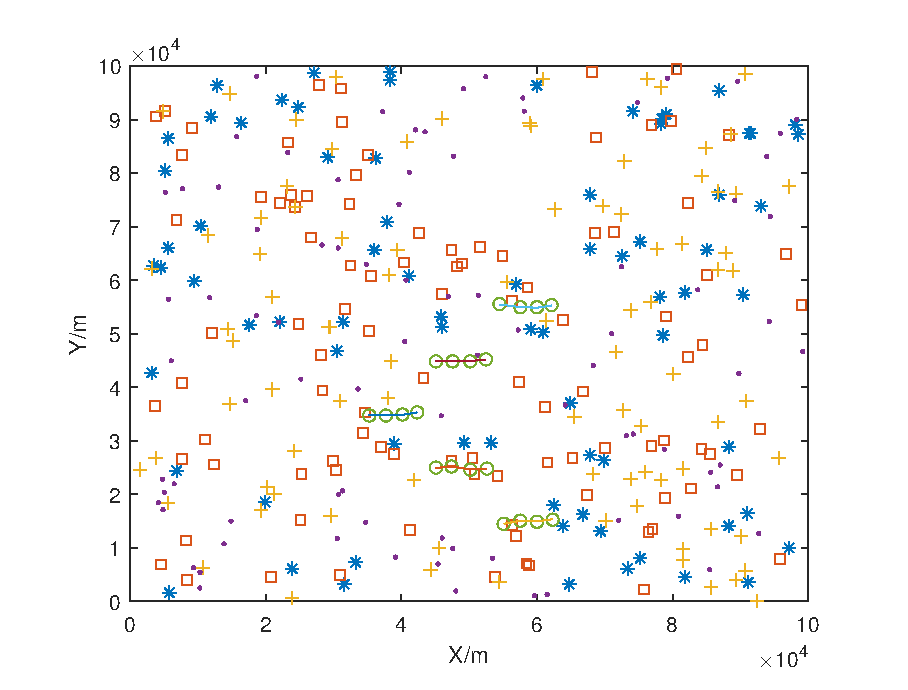
\includegraphics[width=1.2\linewidth]{fig8.eps}
        \caption{Illustration of targets and clutter distributions in detection square.}\label{fig8}
    \end{minipage}
    \begin{minipage}[b]{0.245\textwidth}
        \hspace{-10mm}
        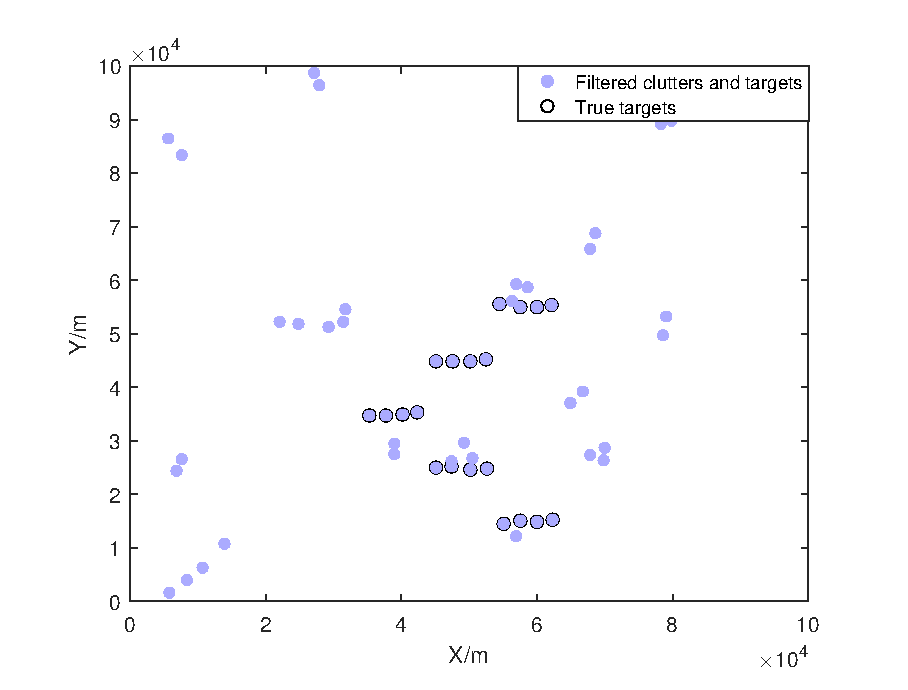
\includegraphics[width=1.2\linewidth]{fig9.eps}
        \caption{The results of the traces extraction based on the extended logic method.}\label{fig9}
    \end{minipage}
    \begin{minipage}[b]{0.245\textwidth}
        \hspace{-7mm}
        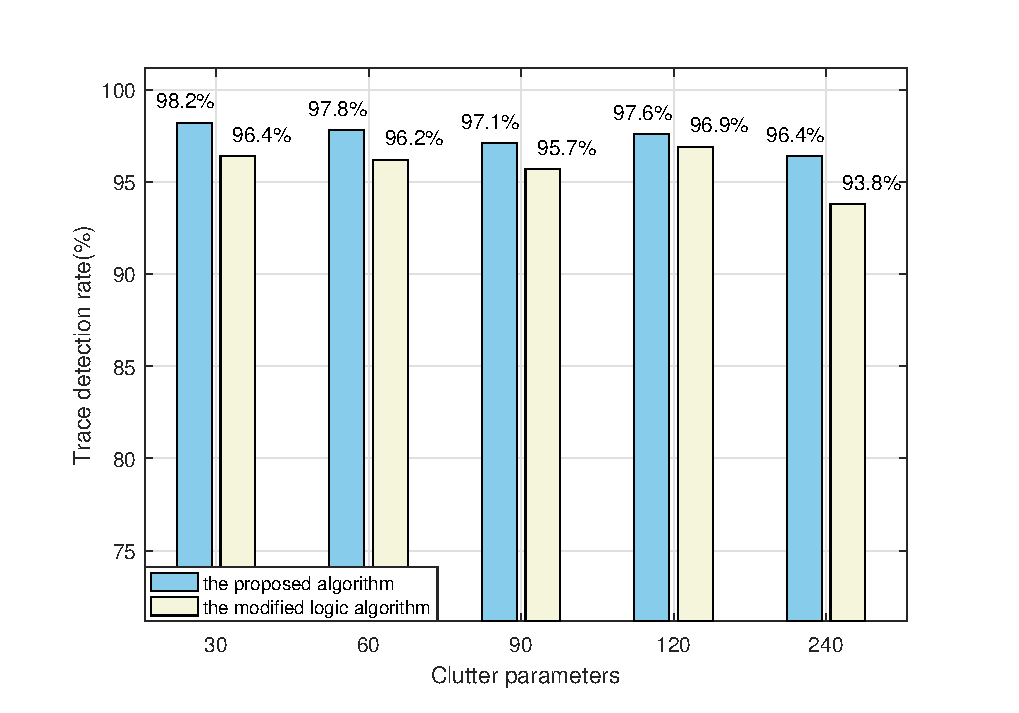
\includegraphics[width=1.15\linewidth,height=0.9\linewidth]{fig10.eps}
        \caption{Trace detection rate of different algorithms under different clutters.}\label{fig10}
    \end{minipage}
    \begin{minipage}[b]{0.245\textwidth}
        \hspace{-7mm}
        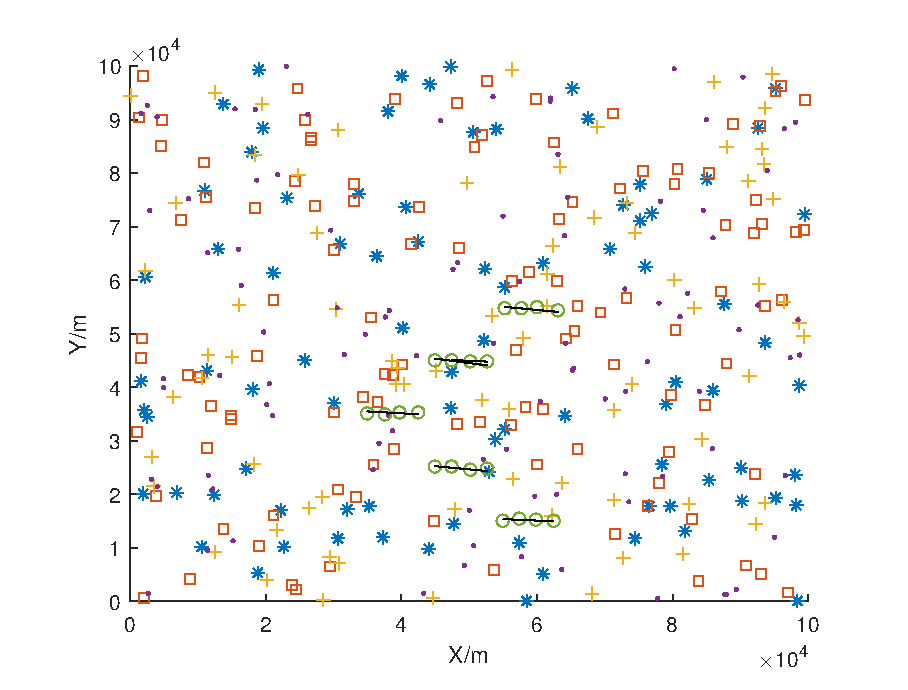
\includegraphics[width=1.2\linewidth]{fig11.eps}
        \caption{The track initiation results of the algorithm proposed.}\label{fig11}
    \end{minipage}
\end{figure*}
\begin{table}[h]
    \vspace{-0.3cm}
    \begin{center}
        \begin{minipage}{\columnwidth}
            \caption{ Multi-objective motion information}\label{tab1}%
            %\begin{tabular*}{\linewidth}{@{}llll@{}}

            \setlength{\tabcolsep}{5mm}{
                \begin{tabular*}{\columnwidth}{@{}cccc@{}}
                    \toprule
                    Target & Initial Position        & Initial Speed              \\
                    \midrule
                    one    & $( 55000 m , 55000 m )$ & $( 500  m / s , 0  m / s)$ \\
                    two    & $( 45000 m , 45000 m )$ & $( 500  m / s , 0  m / s)$
                    \\
                    three  & $( 35000 m , 35000 m )$ & $( 500  m / s , 0  m / s)$ \\
                    four   & $( 45000 m , 25000 m )$ & $( 500  m / s , 0  m / s)$ \\
                    five   & $( 55000 m , 15000 m )$ & $( 500  m / s , 0  m / s)$ \\
                    \botrule
                \end{tabular*}}
            \footnotetext{s = second, m = meter.}
        \end{minipage}
    \end{center}
\end{table}
\vspace{-0.3cm}

\noindent
Errors due to observations from the probing system are that the distance observation variance is $100 m$ and the azimuth observation standard deviation is $0.3  ^ {\circ}$. What's more, the random acceleration perturbation is given to the targets, and they follow the zero-mean Gaussian distribution, and the standard deviation is set to $a_{x}\!=\!1m/s^2$, $a_{y}\!=\!0.6m/s^2$.

Since the clutter positions are random and independent, they can be considered to follow a uniform distribution in the detection square. Therefore, the number of clutter is set to follow the Poisson distribution with the parameter $\lambda$.

The simulation detection system obtains four-cycle measurements in turn, and the detection period is $5s$. The clutters of the four cycles are represented by different symbols, '$\ast$' represents the clutters of the first cycle, and '$\square$' for the second cycle, '+' for the third cycle, '$\cdot$' for the fourth cycle. '$\bigcirc$' represent the true points of the targets. To simulate a strong clutter environment, select $\lambda \!=\!120$. The targets and clutter distributions are shown in Fig. \ref{fig8}.
%\begin{figure}[h]%
% \centering
%\includegraphics[width=0.8\linewidth]{Illustration of targets and clutter distributions.eps}
%  \caption{Illustration of targets and clutter distributions.}\label{fig8}
%\end{figure}
\subsection{Analysis of simulation results}\label{subsec6}

The purpose of the extended logic algorithm is to remove clutters as much as possible, and preserve the true traces of the targets at the same time. So we set the trace detection probability as an indicator to verify the effectiveness of the algorithm.
\begin{equation}\label{eq17}
    P _ { 1 } = \frac { \sum _ { i t = 1 } ^ { M C } N _ { i t } } { M C * N _ { r e a l l y } }
\end{equation}
Where $P_{1}$ represents the trace detection probability, $N_{it}$ represents the number of true tracks detected by the $i_{th}$ experiment. $N_{really}$ represents the number of true traces set per experiment. $M C$ represents the number of times that Monte-Carlo has performed experimental simulations. And the track initiation results after clutter filtering in a Monte-Carlo simulation experiment are shown in Fig. \ref{fig9}.
%\begin{figure}[h]%
%   \centering
%   \includegraphics[width=0.8\linewidth]{The results of the traces extraction.eps}
%   \caption{The results of the traces extraction based on extended logic method.}\label{fig9}
%\end{figure}

100 Monte-Carlo simulation experiments have been performed in different clutter environments. Target maneuver information is set to $v_{max}\!=\!750m/s$, $v_{min}\!=\!333m/s$, $a_{max}\!=\!150m/s^2$, $a_{min}\!=\!0m/s^2$, $v_{tmax}\!=\!6 ^ {\circ}/s$. Select $\gamma\!=\!24$.

In addition, in order to reflect the advantages of the proposed algorithm and the modified logic algorithm \cite{bib21}, the modified logic method was also used to perform 100 Monte-Carlo experiments in the same environment as the control group. The results are shown in Fig. \ref{fig10}. The trace detection rates of the algorithm proposed are stable at around $96 \%$ in different clutter environments, and it performs better than the modified LB method.

%\begin{figure}[h]%
%   \vspace{-0.3cm}
%   \centering
%   \includegraphics[width=0.8\linewidth]{Trace detection rate.eps}
%   \caption{Trace detection rate of different algorithms under different clutters.}\label{fig10}
%\end{figure}
%\vspace{-0.3cm}
In order to show the effect and performance of the algorithm proposed more clearly, the track initiation success rate and the false track occupancy rate are used to characterize the accuracy of the track initiation.
\begin{equation}\label{eq18}
    P _ { 2 } = \frac { \sum _ { i c = 1 } ^ { M C } N _ { i c } } { M C * N _ { r e a l } }
\end{equation}
Where $P_{2}$ represents the track initiation success rate, and $N_{ic}$ represents the number of true tracks that the algorithm successfully initiated by the $i_{th}$ experiment, $N_{real}$ represents the number of targets.
\begin{equation}\label{eq19}
    P _ { 3 } = \frac { \sum _ { i f f = 1 } ^ { M C } N _ { i f } } { \sum _ { t o t a l = 1 } ^ { N } N _ { t o t a l } }
\end{equation}
Where $P_{3}$ represents the false track occupancy rate,$N_{if}$ represents the number of false tracks that the algorithm successfully initiated by the $i_{th}$ experiment, $N_{total}$ represents the number of tracks that the algorithm successfully initiated by the $i_{th}$ experiment.

As for the division of parameter space of the Hough transform, the parameter space is divided into $N_{\rho}\!=\!400$, and $N_{\theta}\!=\!200$. The threshold coefficients are set to $p\!=\!0.5$, $q\!=\!0.68$. 100 Monte-Carlo simulation experiments are performed by the algorithm proposed in this paper in different clutter environments. The track initiation result of a Monte-Carlo simulation experiment is shown in Fig. \ref{fig11}. And the black lines represent the tracks successfully initiated.
%\begin{figure}[h]%
%  \centering
%   \includegraphics[width=0.8\linewidth]{The track initiation results of the algorithm proposed.eps}
%   \caption{The track initiation results of the algorithm proposed.}\label{fig11}
%\end{figure}

And the modified Hough transform (modified HT) \cite{bib22} was also used to perform 100 Monte-Carlo experiments in the same environment as the control group. For the modified HT, only three beats of measurements are set, so $N\!=\!3$, $\lambda\!=\!120$, and set $v_{max}\!=\!750m/s$, $v_{min}\!=\!333m/s$. The results are shown in Fig. \ref{fig12}.
\begin{figure}[h]%
    \vspace{-0.5cm}
    \setlength{\abovedisplayskip}{-0.2cm}
    \setlength{\belowcaptionskip}{-1cm}
    \centering
    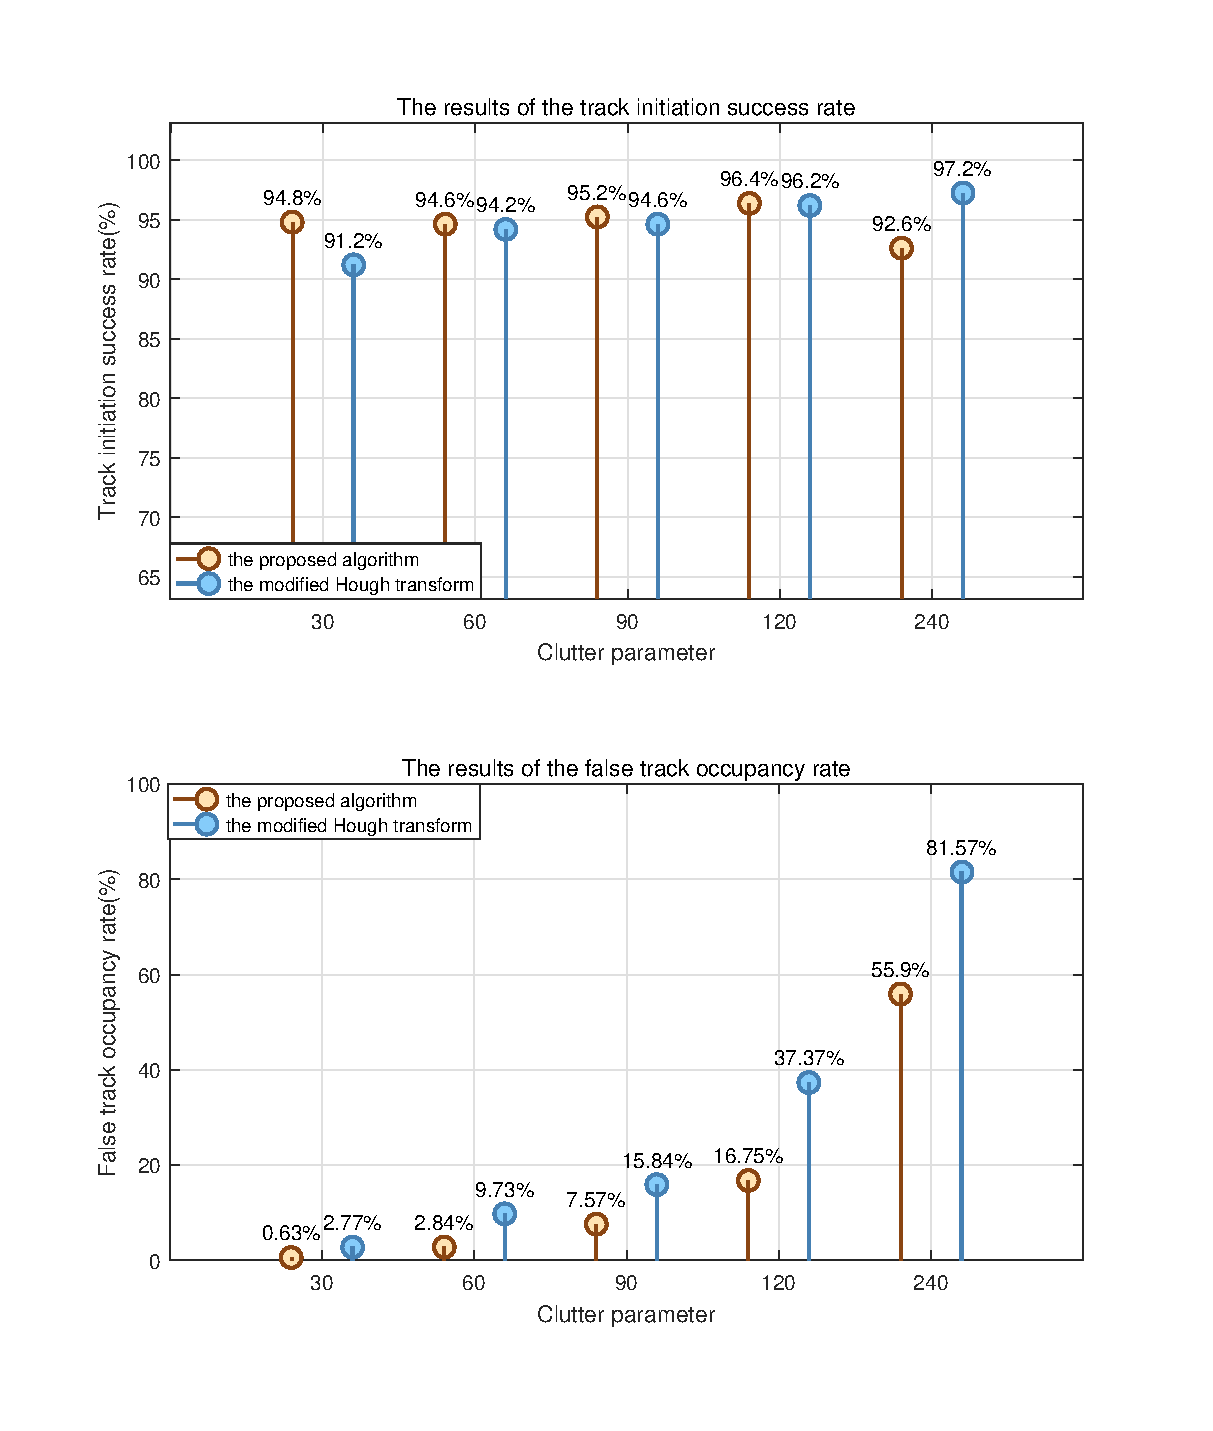
\includegraphics[width=0.38\textwidth]{fig12.eps}
    \caption{Track initiation quality of different algorithms under different clutter.}\label{fig12}
\end{figure}

Compared to the track start success rates with modified HT, the proposed algorithm performs well in different clutter environments, while the initiation success rate is slightly lower than the modified HT under strong clutter. Even as clutters increase, the modified HT shows a higher and higher initial success rate. However, as the clutter increases, so do the false tracks. And the false tracks occupancy rate of the proposed algorithm can basically remain about half of the modified HT.

What's more, 100 simulation experiments are performed on the modified Logic-Based method (modified LB), the sequence Hough transform algorithm (SHT) \cite{bib23}, and the fuzzy parallel Hough transform (FPHT) \cite{bib13} respectively. The SHT is divided into two kinds of simulation experiments: the sequence Hough transform for short initiation beats (SHT-S) and the sequence Hough transform for long initiation beats (SHT-L). For the SHT-S, we set the initiation beats $N\!=\!4$, clutter parameter $\lambda\!=\!120$, and the number of sequences is $6$. For the SHT-L, set the initiation beats $N\!=\!12$, clutter parameters $\lambda\!=\!30$, and the number of sequences is also $6$. As for the FPHT, clutter parameters $\lambda\!=\!50$, and set the threshold is $0.75$ of the accumulative peak. And the results are shown in Table \ref{tab2}.
\begin{table}[t]
    \begin{center}
        \begin{minipage}{\linewidth}
            \caption{Comparison of track initiation results for different algorithms}\label{tab2}
            %\begin{tabular*}{\linewidth}{@{\extracolsep{\fill}}lcccccc@
            % {\extracolsep{\fill}}}
            \setlength{\tabcolsep}{1mm}{
                \begin{tabular*}{\textwidth}{@{}lccccccc@{}}
                    \toprule%
                    Method & beats & $\lambda$ & $P_{1}$  & $P_{2}$  & $P_{3}$   & $Time(s)$ \\
                    \midrule
                    SHT-S  & 4     & 120       & $39.1\%$ & $25.4\%$ & $78.83\%$ & 3.28      \\
                    SHT-L  & 12    & 30        & $79.2\%$ & $82.8\%$ & $31.72\%$ & 2.97      \\
                    SHT*\footnotemark[1] & 10    & 50        & /\       & $85.7\%$ & $20.32\%$ & 12.31     \\
                    FPHT    & 4     & 50        & $90.2\%$ & $82.6\%$ & $93.29\%$ & 15.54     \\
                    modified LB   & 4     & 120       & $96.9\%$ & $92.6\%$ & $63.95\%$ & 0.25      \\
                    modified HT  & 3     & 120       & $93.5\%$ & $96.2\%$ & $37.37\%$ & 0.38      \\
                    ours   & 4     & 120       & $97.6\%$ & $96.4\%$ & $16.75\%$ & 3.76      \\
                    \botrule
                \end{tabular*}}
            \footnotetext[1]{ SHT* represents the data in this row is the experimental result data given by the corresponding literature. $P_{1}$ is not used as an evaluation index in the original reference, so the $P_{1}$ index in this row is empty. The original reference is old, and the hardware environment is different, the running time of this row is not included in the comparison range. }
        \end{minipage}
    \end{center}
\end{table}

Comparing the average running time of different algorithms, we find that the logic method has the fastest speed, while FPHT has a relatively high amount of calculation because it uses Gaussian functions for membership calculation. The algorithm proposed combines the general LB and HT method, so the amount of calculation is increased. However, in the process of introducing fuzzy theory, the process of the Hough transformation is greatly simplified. Therefore, it can be considered to have a middle amount of operation.

Compared to the algorithm proposed to others, we can see that although the modified LB can achieve a high track initiation success rate, the false track occupancy rate is too high.

Because the initiation beats are too short, and the clutters cause a huge amount of interference, the track initiation success rate of SHT-S is very low. For the SHT-L, it has a high track initiation success rate, and at the same time, compared to modified LB, there is a significant reduction in false tracks. However, if you want to use SHT to complete a high-quality track initiation as shown in the SHT* results, you must take a long initiation time and the clutter and noise should not be too strong. Therefore, the initiation time of SHT is too long, limited by the number of sequences, and sensitive to noise, it is unsuitable for track initiation under strong clutter.

Regarding the FPHT, even in a low clutter environment, its track initiation success rate is not particularly high. While not requiring any prior information is a great advantage, it causes a lot of fake tracks.

For modified HT, although it can complete a high-quality initiation with a short initiation time and has fewer false tracks than the modified LB, this method can only use the first three beats of the measurements, which has great limitations and is only suitable for the track initiation with high detection rates.

The algorithm proposed has a higher track initiation success rate, and a lower false track occupancy rate in a short period of time. Therefore, it is believed that under the strong clutter, it has a higher quality track initiation ability.

\section{Conclusion}\label{sec4}

For the existing algorithm of track initiation in a strong clutter environment, there are too many false tracks and low initiation quality in complex environments. Based on adaptive gates and fuzzy Hough transform, a track initiation algorithm is proposed. A new Hough transform rule is designed to reduce the invalid accumulation within the same detection cycle. The simulation results show that the algorithm proposed not only guarantees the high-quality track initiation in a shorter time, but also reduces the false track occupancy rate, which is more suitable for multi-target track initiation problems in complex environments. Reducing the amount of computation and completing great initiation quality at low detection rates are the next phase of work objectives.

\section*{Declarations}

\subsection*{Ethical Approval}
Not applicable.

\subsection*{Competing interests}
The authors declare that they have no competing financial interests.

\subsection*{Authors' contributions}
Liu Zeng: Investigation, Methodology, formal analysis, Writing original draft; Gang Xiao: Project administration, Writing review \& editing; Chunshan Ding: Conceptualization, resources. Yangguang He: Supervision, Data curation.

\subsection*{Funding}
This paper is sponsored by National Natural Science Foundation of China (61673270; 61973212) and Science and Technology Project of Zhejiang Province (2022C01013).

\subsection*{Availability of data and materials}
The datasets used or analysed during the current study are available from the corresponding author on reasonable request.

\bibliographystyle{sn-standardnature}
\bibliography{ref}% common bib file


%% if required, the content of .bbl file can be included here once bbl is generated
%%\input sn-article.bbl

%% Default %%
%%\input sn-sample-bib.tex%

\end{document}



